\documentclass[border=4pt]{standalone}
\usepackage{amsmath,amssymb}
\usepackage{tikz}
\begin{document}
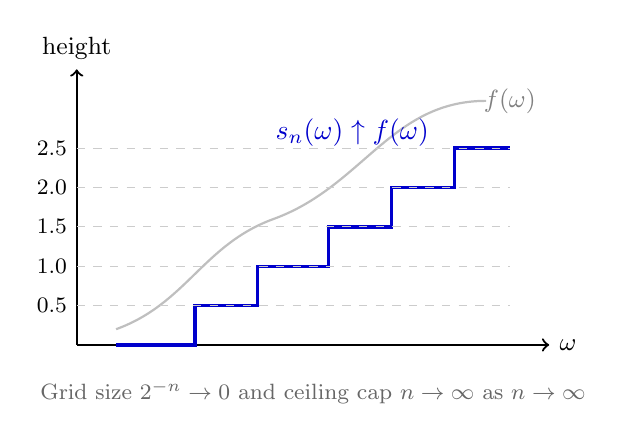
\begin{tikzpicture}[font=\small]
  \draw[->, thick] (0,0) -- (6.0,0) node[right] {$\omega$};
  \draw[->, thick] (0,0) -- (0,3.5) node[above] {height};
  
  % True function f
  \draw[thick, gray!50, smooth] (0.5,0.2) to[out=20,in=200] (2.5,1.6) to[out=20,in=180] (5.2,3.1);
  \node[gray] at (5.5, 3.1) {$f(\omega)$};

  % Staircase s_n
  \draw[very thick, blue!80!black] (0.5, 0.0) -- (1.5, 0.0)
    -- (1.5, 0.5) -- (2.3, 0.5)
    -- (2.3, 1.0) -- (3.2, 1.0)
    -- (3.2, 1.5) -- (4.0, 1.5)
    -- (4.0, 2.0) -- (4.8, 2.0)
    -- (4.8, 2.5) -- (5.5, 2.5);
  \node[blue!80!black, font=\bfseries] at (3.5, 2.7) {$s_n(\omega) \uparrow f(\omega)$};

  \foreach \y in {0.5, 1.0, 1.5, 2.0, 2.5} {
    \draw[dashed, gray!40] (0, \y) -- (5.5, \y);
    \node[left, font=\footnotesize] at (0,\y) {$\y$};
  }
  \node[font=\footnotesize, text=gray!80!black] at (3.0, -0.6) 
    {Grid size $2^{-n} \to 0$ and ceiling cap $n \to \infty$ as $n \to \infty$};
\end{tikzpicture}
\end{document}